%%%%%%%%%%%%%%%%%%%%%%%%%%%%%%%%%%%%%%%%%%%%%%%%%%%%%%%%%%%%%%%%%%%%
% Grundlagen
%%%%%%%%%%%%%%%%%%%%%%%%%%%%%%%%%%%%%%%%%%%%%%%%%%%%%%%%%%%%%%%%%%%%

\chapter{Material and Methods}
  \label{MatMet}

\noindent
In this chapter ...

\section{Title of section}
  \label{Abschnittslabel} 

BlaBlaBla ...

\subsection{Title of subsection}
  \label{Unterabschnittslabel}

BlaBlaBla ...

Zum Einbinden einer Abbildung mittels `pdf-Datei' in ein
\LaTeX-Dokument benutzt man folgenden \LaTeX-Code:

\begin{verbatim}
\begin{figure}[htb]
     \centerline{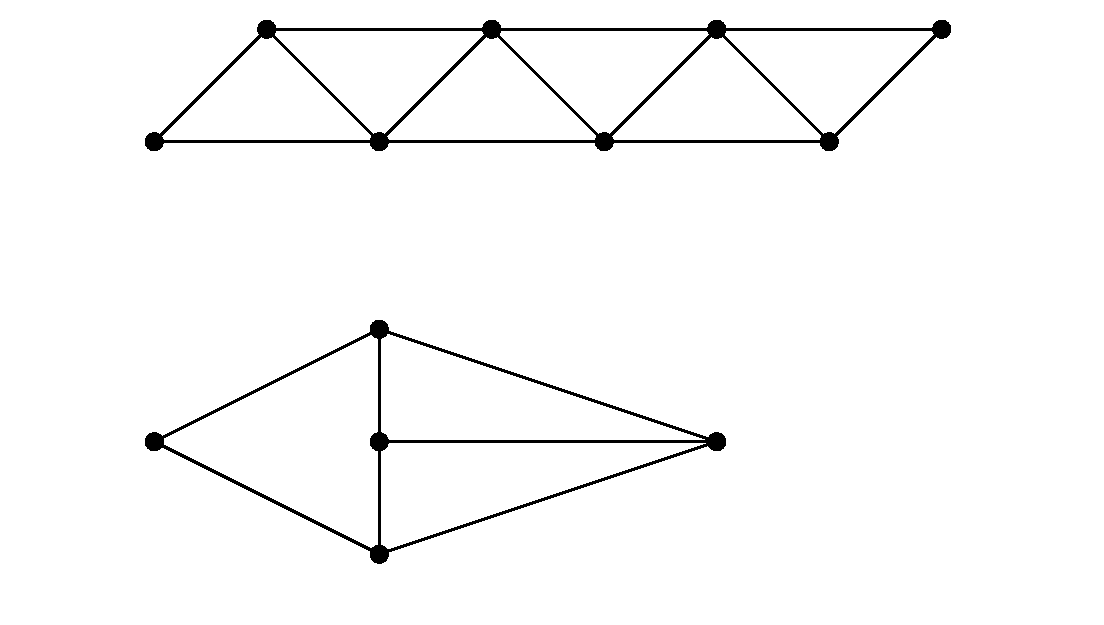
\includegraphics{figures/chordal.pdf}}
  \caption{Chordale Graphen}
  \label{chordal}
\end{figure}
\end{verbatim}

\begin{figure}[htb]
     \centerline{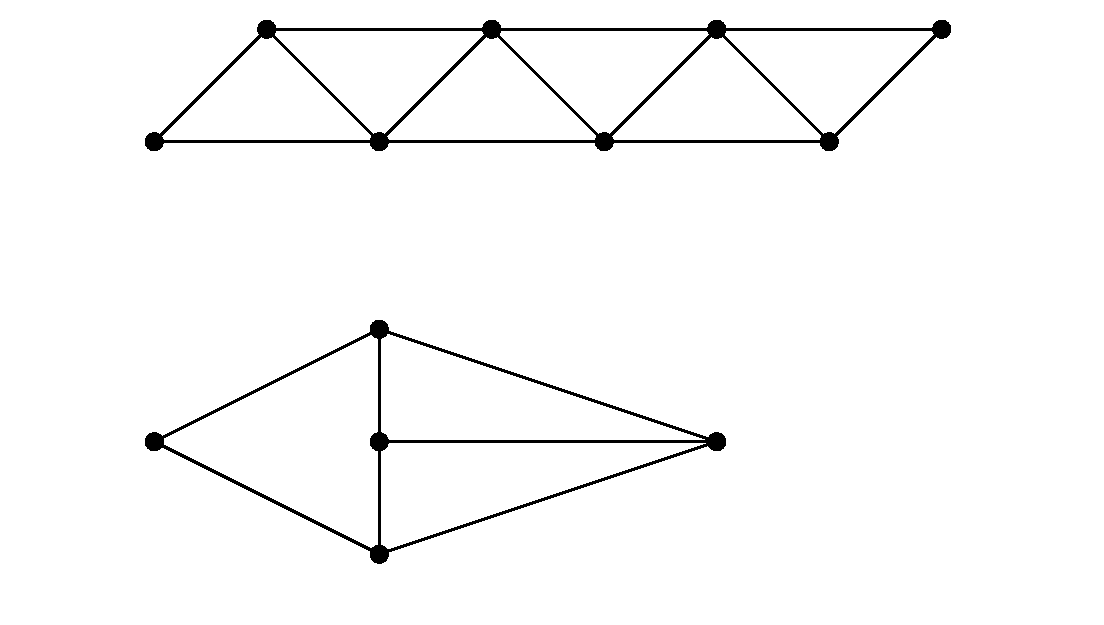
\includegraphics{figures/chordal.pdf}}
  \caption{Chordal Graphs}
  \label{chordal}
\end{figure}

Abbildung~\ref{chordal} zeigt ...

Tabellen k\"onnen wie folgt erstellt werden:

{
\renewcommand{\baselinestretch}{0.9} 
\normalsize
\begin{table}[htb]
\begin{tabular}{|p{2.7cm}||l|c|r|}
\hline
    \textbf{Spalte 1} 
  & \textbf{Spalte 2} 
  & \textbf{Spalte 3} 
  & \textbf{Spalte 4} \\
  \hline\hline
  xxx1111
  & xxxxxxx2222222
  & xxxxxx333333 
  & xxxxxxxxxx444444 \\
  \hline
    ...
  & ...
  & ...
  & ...\\
  \hline
\end{tabular}
  \caption[Diese Kurzcaption ist fuer das Tabellenverzeichnis]{Beispieltabelle mit einer langen Legende, damit man sieht, dass in der Legende der Zeilenabstand verringert wurde. Ausserdem soll auch der Font etwas kleiner gew\"ahlt werden. So sieht die ganze Umgebung kompakter aus.}
  \label{tabelle-1}
\end{table}
}

\noindent
Eine Aufz\"ahlung geht wie folgt:
\begin{itemize}
\item ...
\item ...
\end{itemize}
Eine numerierte Aufz\"ahlung:
\begin{enumerate}
\item ...
\item ...
\end{enumerate}

Betonungen sollen \emph{kursiv} gedruckt werden. 
\textbf{Fettdruck} ist auch m\"oglich.

Referenzen: \cite{SaaSchTue97,TueConSaa96ismis,SchTueSaa98preprint}
